\documentclass{beamer}

\begin{document}

\begin{frame}
\frametitle{Transformare adiabatică}
\end{frame}

\begin{frame}
\frametitle{Ecuația transformării adiabatice}
Transformarea adiabatică a gazului ideal poate fi descrisă de ecuația:
\begin{equation}
pV^{\gamma} = \text{constant}
\end{equation}
unde $p$ este presiunea, $V$ este volumul, iar (doar pentru gaze perfecte):
\begin{equation}
\gamma = \frac{C_p}{C_v} = \frac{i+2}{i}
\end{equation}
\end{frame}

\begin{frame}
\frametitle{Curba ce reprezintă variația presiunii în funcție de volum}
\begin{figure}
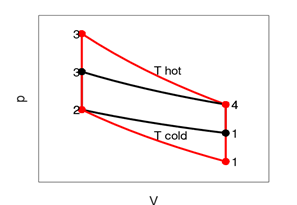
\includegraphics[width=\textwidth]{Picture1.png}
\end{figure}
\end{frame}

\begin{frame}
\frametitle{Concluzii}
Transformarea adiabatică este un proces termodinamic în care sistemul termodinamic se schimbă dintr-o stare inițială într-o altă stare finală, fără a exista transfer de căldură între sistem și mediul extern. Acest lucru înseamnă că sistemul termodinamic nu primește nicio cantitate de căldură de la mediul extern și nici nu cedează căldură către mediul extern.

\end{frame}

\end{document}